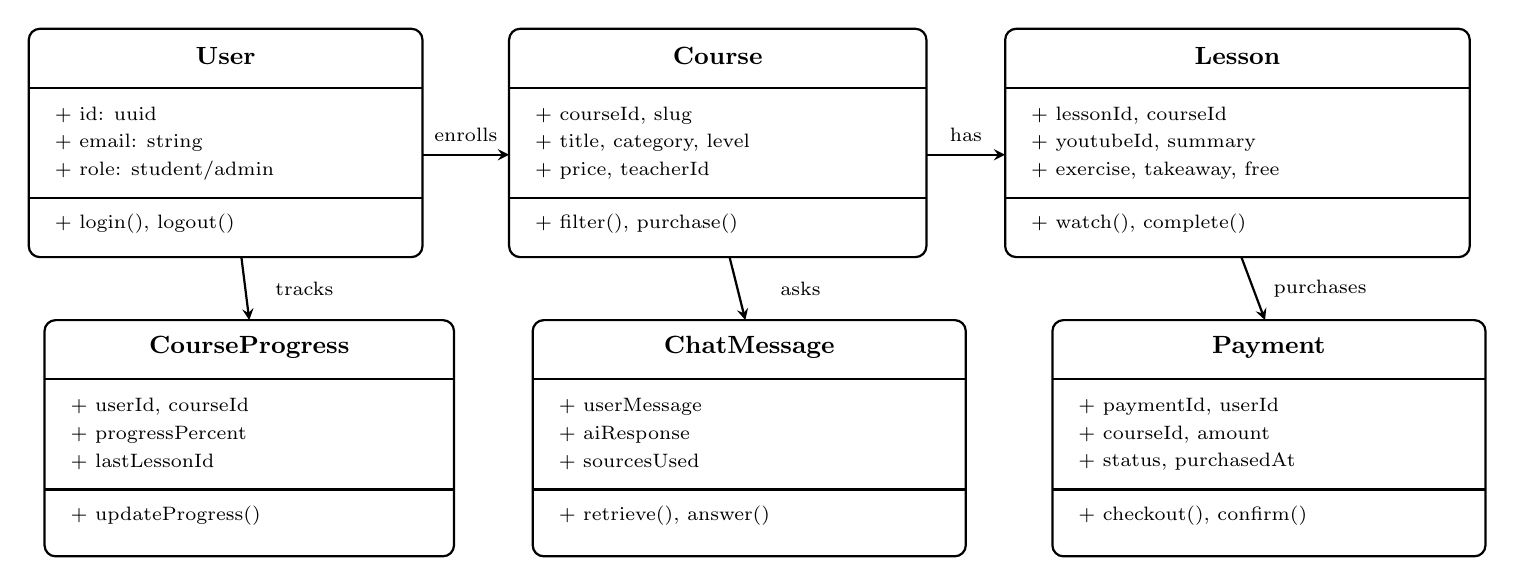
\begin{tikzpicture}[x=1cm,y=1cm,>=stealth,thick]
  \draw[rounded corners=4pt] (0,6.3) rectangle (5.0,9.2);
  \node[font=\small\bfseries] at (2.5,8.85) {User};
  \draw (0,8.45) -- (5.0,8.45);
  \node[anchor=west,font=\scriptsize] at (0.2,8.1) {+ id: uuid};
  \node[anchor=west,font=\scriptsize] at (0.2,7.75) {+ email: string};
  \node[anchor=west,font=\scriptsize] at (0.2,7.4) {+ role: student/admin};
  \draw (0,7.05) -- (5.0,7.05);
  \node[anchor=west,font=\scriptsize] at (0.2,6.72) {+ login(), logout()};

  \draw[rounded corners=4pt] (6.1,6.3) rectangle (11.4,9.2);
  \node[font=\small\bfseries] at (8.75,8.85) {Course};
  \draw (6.1,8.45) -- (11.4,8.45);
  \node[anchor=west,font=\scriptsize] at (6.3,8.1) {+ courseId, slug};
  \node[anchor=west,font=\scriptsize] at (6.3,7.75) {+ title, category, level};
  \node[anchor=west,font=\scriptsize] at (6.3,7.4) {+ price, teacherId};
  \draw (6.1,7.05) -- (11.4,7.05);
  \node[anchor=west,font=\scriptsize] at (6.3,6.72) {+ filter(), purchase()};

  \draw[rounded corners=4pt] (12.4,6.3) rectangle (18.3,9.2);
  \node[font=\small\bfseries] at (15.35,8.85) {Lesson};
  \draw (12.4,8.45) -- (18.3,8.45);
  \node[anchor=west,font=\scriptsize] at (12.6,8.1) {+ lessonId, courseId};
  \node[anchor=west,font=\scriptsize] at (12.6,7.75) {+ youtubeId, summary};
  \node[anchor=west,font=\scriptsize] at (12.6,7.4) {+ exercise, takeaway, free};
  \draw (12.4,7.05) -- (18.3,7.05);
  \node[anchor=west,font=\scriptsize] at (12.6,6.72) {+ watch(), complete()};

  \draw[rounded corners=4pt] (0.2,2.5) rectangle (5.4,5.5);
  \node[font=\small\bfseries] at (2.8,5.15) {CourseProgress};
  \draw (0.2,4.75) -- (5.4,4.75);
  \node[anchor=west,font=\scriptsize] at (0.4,4.4) {+ userId, courseId};
  \node[anchor=west,font=\scriptsize] at (0.4,4.05) {+ progressPercent};
  \node[anchor=west,font=\scriptsize] at (0.4,3.7) {+ lastLessonId};
  \draw (0.2,3.35) -- (5.4,3.35);
  \node[anchor=west,font=\scriptsize] at (0.4,3.02) {+ updateProgress()};

  \draw[rounded corners=4pt] (6.4,2.5) rectangle (11.9,5.5);
  \node[font=\small\bfseries] at (9.15,5.15) {ChatMessage};
  \draw (6.4,4.75) -- (11.9,4.75);
  \node[anchor=west,font=\scriptsize] at (6.6,4.4) {+ userMessage};
  \node[anchor=west,font=\scriptsize] at (6.6,4.05) {+ aiResponse};
  \node[anchor=west,font=\scriptsize] at (6.6,3.7) {+ sourcesUsed};
  \draw (6.4,3.35) -- (11.9,3.35);
  \node[anchor=west,font=\scriptsize] at (6.6,3.02) {+ retrieve(), answer()};

  \draw[rounded corners=4pt] (13.0,2.5) rectangle (18.5,5.5);
  \node[font=\small\bfseries] at (15.75,5.15) {Payment};
  \draw (13.0,4.75) -- (18.5,4.75);
  \node[anchor=west,font=\scriptsize] at (13.2,4.4) {+ paymentId, userId};
  \node[anchor=west,font=\scriptsize] at (13.2,4.05) {+ courseId, amount};
  \node[anchor=west,font=\scriptsize] at (13.2,3.7) {+ status, purchasedAt};
  \draw (13.0,3.35) -- (18.5,3.35);
  \node[anchor=west,font=\scriptsize] at (13.2,3.02) {+ checkout(), confirm()};

  \draw[->] (5.0,7.6) -- (6.1,7.6);
  \node[font=\scriptsize, fill=white, inner sep=1pt] at (5.55,7.85) {enrolls};
  \draw[->] (11.4,7.6) -- (12.4,7.6);
  \node[font=\scriptsize, fill=white, inner sep=1pt] at (11.9,7.85) {has};
  \draw[->] (2.7,6.3) -- (2.8,5.5);
  \node[font=\scriptsize, fill=white, inner sep=1pt] at (3.5,5.9) {tracks};
  \draw[->] (8.9,6.3) -- (9.1,5.5);
  \node[font=\scriptsize, fill=white, inner sep=1pt] at (9.8,5.9) {asks};
  \draw[->] (15.4,6.3) -- (15.7,5.5);
  \node[font=\scriptsize, fill=white, inner sep=1pt] at (16.4,5.9) {purchases};
\end{tikzpicture}
